\documentclass{standalone}
\usepackage{tikz}
\usetikzlibrary{arrows.meta, positioning, shapes.geometric, calc,patterns}

\begin{document}
	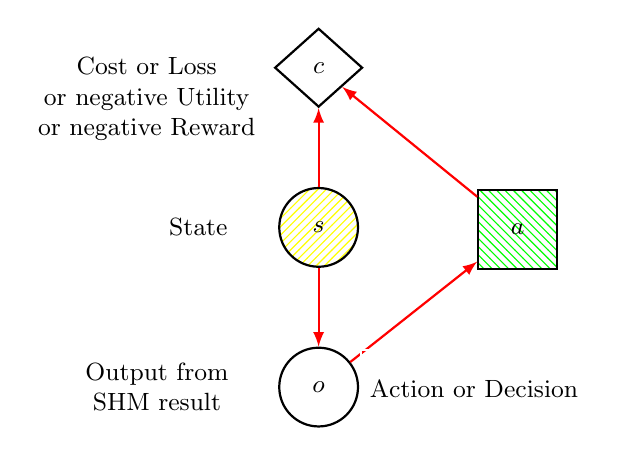
\begin{tikzpicture}[
		node distance=2cm and 1.5cm,
		every node/.style={minimum size=10mm, font=\small},
		cost/.style={draw,diamond, aspect=2, fill=white},
		state/.style={draw,circle,pattern=north east lines, pattern color=yellow},
		obs/.style={draw,circle, fill=white},
		action/.style={draw,rectangle, ,pattern=north west lines, pattern color=green},
		->, >=Stealth, thick, black
		]
		% Simple Influence diagram
		\node[cost] at (0,0) (cost) {$c$};
		\node[state, below = of cost, yshift = 10mm] (state) {$s$};
		\node[obs,below = of state, yshift = 10mm] (obs) {$o$};
		\node[action,right = of obs,yshift = 20mm] (action) {$a$};
%		\node[obs] at (0,0) (obs) {$o$};	
%		\node[action, right = of obs] (action){$a$};
%		\node[state, below = of obs] (state){$s$};
%		\node[cost, right = of state] (cost) {$c$};
%		
		% Draw the causality arrows
		\draw[-latex,red] (obs)--(action);
		\draw[-latex,red] (action) -- (cost);
		\draw[-latex,red] (state) -- (cost);
		\draw[-latex,red] (state) -- (obs);
		% denote
		\node[draw = white,left= of cost,align=center,xshift= 14mm,yshift = -4mm]  {Cost or Loss \\ or negative Utility \\or negative Reward};
		
		\node[draw = white, left = of state,align = center,xshift= 10mm] {State};
		
		\node[draw = white, left = of obs,align = center,xshift= 10mm]  {Output from \\ SHM result};
		
		\node[draw = white, below = of action, align=center,xshift= -5mm,yshift= 10mm] {Action or Decision };

		
	\end{tikzpicture}
\end{document}
